% Standalone RAKL transfer-ladder diagram (Paper II).
% retrieved source  !=  witnessed applicability  !=  verified success.
% This paper studies the MIDDLE stage.
% Build:  pdflatex transfer_ladder.tex  -> transfer_ladder.pdf
\documentclass[border=6pt]{standalone}
\usepackage{amsmath}
\usepackage{tikz}
\usepackage{helvet}\renewcommand{\familydefault}{\sfdefault}
\usetikzlibrary{positioning,arrows.meta,shapes.geometric,fit,backgrounds,calc}
\definecolor{oiblue}{RGB}{0,114,178}
\definecolor{oiverm}{RGB}{213,94,0}
\begin{document}
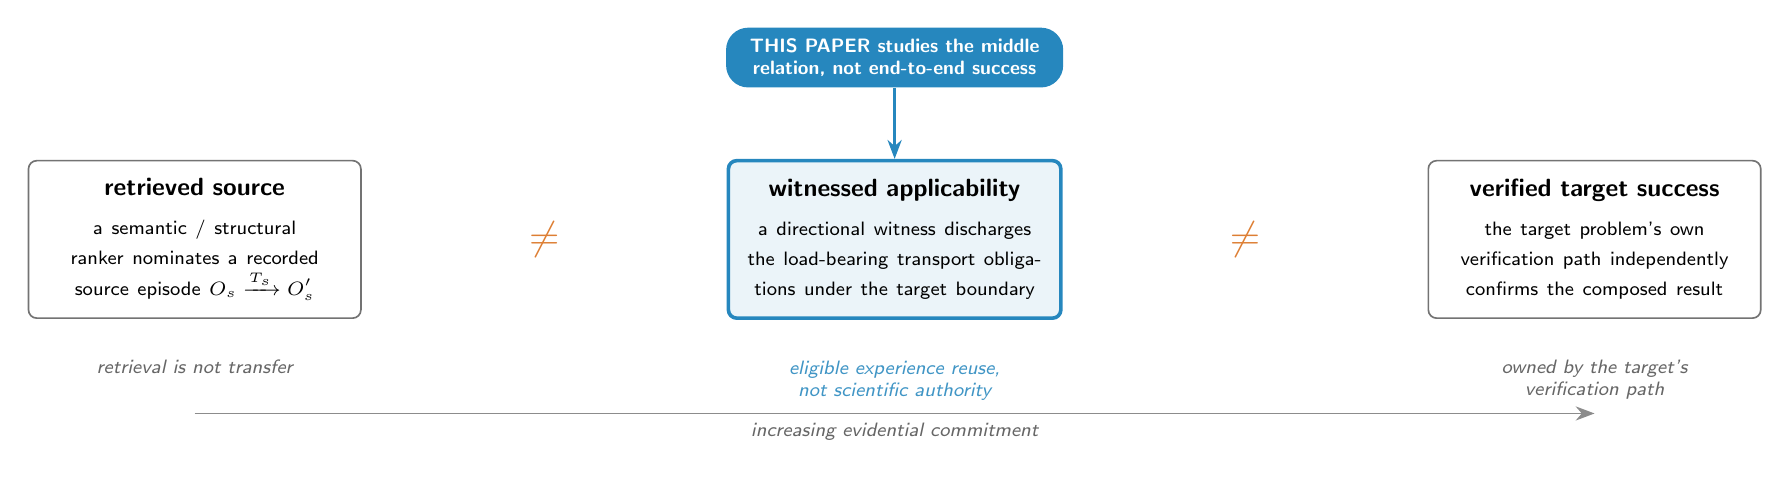
\begin{tikzpicture}[
  font=\small,
  >={Stealth[length=2.4mm]},
  stage/.style={rounded corners=3pt, draw=black!55, line width=0.6pt, align=center,
               inner sep=6pt, minimum height=20mm, text width=38mm, fill=white},
  focus/.style={rounded corners=3pt, draw=oiblue!85, line width=1.3pt, align=center,
               inner sep=6pt, minimum height=20mm, text width=38mm, fill=oiblue!8},
  neq/.style={font=\Large\bfseries, text=oiverm!80},
  lbl/.style={font=\scriptsize\itshape, text=black!60, align=center},
  node distance=20mm,
]

% ---- three stages ----
\node[stage] (src)
  {\textbf{retrieved source}\\[3pt]
   {\scriptsize a semantic / structural ranker nominates a recorded source episode
    $O_s\!\xrightarrow{T_s}\!O_s'$}};
\node[neq, right=of src] (n1) {$\neq$};
\node[focus, right=of n1] (app)
  {\textbf{witnessed applicability}\\[3pt]
   {\scriptsize a directional witness discharges the load-bearing transport
    obligations under the target boundary}};
\node[neq, right=of app] (n2) {$\neq$};
\node[stage, right=of n2] (succ)
  {\textbf{verified target success}\\[3pt]
   {\scriptsize the target problem's own verification path independently confirms
    the composed result}};

% ---- stage undercaptions ----
\node[lbl, below=4mm of src] {retrieval is not transfer};
\node[lbl, below=4mm of app, text=oiblue!75] {eligible experience reuse,\\not scientific authority};
\node[lbl, below=4mm of succ] {owned by the target's\\verification path};

% ---- "this paper studies the middle stage" marker ----
\node[rounded corners=8pt, fill=oiblue!85, text=white, font=\scriptsize\bfseries,
      inner sep=4pt, text width=40mm, align=center, above=9mm of app] (mark)
   {THIS PAPER studies the middle relation, not end-to-end success};
\draw[->, line width=1.0pt, draw=oiblue!85] (mark) -- (app.north);

% ---- forward progression arrows along the bottom ----
\begin{scope}[on background layer]
  \draw[->, line width=0.6pt, draw=black!45]
     ($(src.south)-(0,12mm)$) -- node[lbl, below]{increasing evidential commitment}
     ($(succ.south)-(0,12mm)$);
\end{scope}

\end{tikzpicture}
\end{document}
